\subsection{Does the first range-label gain require new structures?}
A post-hoc control separates two changes that occurred together in the first
round: adding newly evaluated structures and redefining their energy classes.
This follow-up was prompted by the first-round result; it is a mechanistic
test, not a new blind confirmation. Its plan and paired fit/proposal seeds were
frozen before the follow-up fits.

For each architecture and each of the three seeds, the comparison starts from
the same original 4,000-update checkpoint and allocates another 2,000 updates.
The original H0 data and first-round augmented data are each evaluated with
fixed bins and with identical range-bin edges. Existing equal-update
checkpoints supply the H0/fixed and augmented-data comparisons. We additionally
fit H0 with range edges estimated from H0 TRAIN alone, which tests relabeling
without any acquired labels. Some H0 and augmented-data range edges differ,
so six more H0 fits use each lineage's exact first-round range edges. These
remove edge location as a difference when testing the effect of added rows.
There are twelve new fits in total; all requested classes have actual H0
TRAIN support.

All compared checkpoints generate fresh proposals under one common history,
with 128 attempts for each count/request cell and common proposal streams.
Their energies are evaluated under the original, teacher-specific H0
assessment bins. None of these assessment labels enter training. The
comparison therefore asks whether new rows help under the same physical
energy intervals, rather than allowing the assessment target to move.

\begin{table}[htbp]
\centering\small
\caption{Posthoc conditioning/data controls: balanced H0 fixed-bin yield change, percentage points, mean $\pm$ sample SD over three paired fits. Relabeling also changes class-balanced loss weights. The matched-range comparison holds the physical edges identical; adding rows can still change minibatches and row weights.}
\begin{tabular}{lrr}\toprule
Model / contrast & UMA & MACE\\\midrule
AR / H0 range versus fixed & $+6.48\pm1.01$ & $+6.11\pm0.98$\\
AR / New rows / fixed edges & $-1.56\pm0.88$ & $-1.10\pm1.33$\\
AR / New rows / matched range edges & $-1.36\pm0.39$ & $-2.05\pm0.84$\\
CVAE $D=2$ / H0 range versus fixed & $+7.06\pm1.09$ & $+6.80\pm0.91$\\
CVAE $D=2$ / New rows / fixed edges & $+0.41\pm0.78$ & $+0.09\pm0.46$\\
CVAE $D=2$ / New rows / matched range edges & $+1.85\pm1.33$ & $+2.00\pm1.39$\\
\bottomrule\end{tabular}
\end{table}


Relabeling H0 alone recovers a large gain: $+6.48\pm1.01$ percentage points for
AR and $+7.06\pm1.09$ for $D=2$ under UMA. MACE gives
$+6.11\pm0.98$ and $+6.80\pm0.91$ points. The corresponding effect of adding
rows at identical first-round range edges is smaller and depends on the
architecture: $-1.36\pm0.39$ points for AR and $+1.85\pm1.33$ for $D=2$
under UMA, with MACE changes of $-2.05\pm0.84$ and $+2.00\pm1.39$.
Under the original fixed bins, adding rows changes UMA yield by
$-1.56\pm0.88$ for AR and $+0.41\pm0.78$ for $D=2$.
These are sample SDs over three paired fit/proposal replicates.

The large first-round gain can thus be obtained without acquiring new
structures. This supports a useful role for the definition of the conditioning
classes and the associated loss weighting. It does not establish that
acquisition is useless: added rows have a small positive effect for $D=2$
under matched range edges, and the acquisition pools extend the observed
upper-energy range. Nor does the control isolate why relabeling helps.
Relabeling changes class membership and the weights assigned by the
class-balanced loss; adding rows also changes minibatches and class weights.
The effects measured here belong to that declared training procedure.

\begin{figure}[htbp]
\centering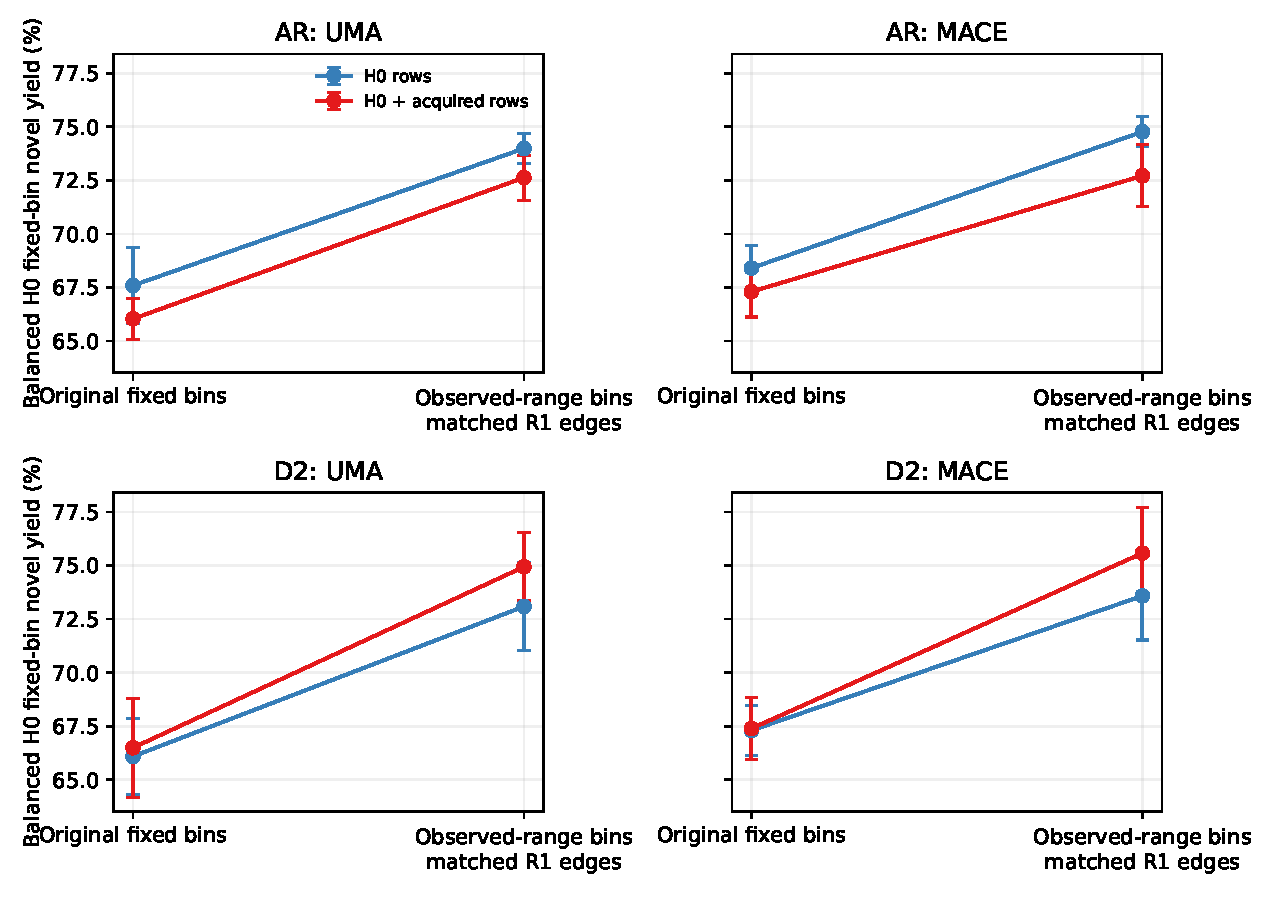
\includegraphics[width=\linewidth]{causal_factorial.pdf}
\caption{Post-hoc data-by-conditioning control on fresh common proposals.
The two data choices use identical physical condition edges at each plotted
position. The separate pure-H0 range fit, whose edges need no acquired labels,
is included in the control table. Error bars show three-pair sample SD.
The result concerns fixed-H0 conditional yield, not DFT accuracy or a
global energy minimum.}
\end{figure}

The follow-up completes in 18.04 minutes and uses 34,686 geometry--teacher
evaluations, with all raw-score checks passing. Its raw proposal identities
are reserved before the subsequent search pilot, preserving the assessment
boundary.
